%\newpage
%\thispagestyle{plain}
%\ifthenelse {\boolean{bachelor}}
%{
%	%\section{Technical documentation}
%	\section{Technická dokumentácia}
%}
%{
%	%\chapter{Technical documentation}
%	\chapter{Technická dokumentácia}
%}
% \label{technical_documentation}
%Lorem ipsum dolor sit amet, consectetuer adipiscing elit, sed diam nonummy nibh euismod tincidunt ut laoreet dolore magna aliquam erat volutpat. Ut wisi enim ad minim veniam, quis nostrud exerci tation ullamcorper suscipit lobortis nisl ut aliquip ex ea commodo consequat. 
%\ifthenelse {\boolean{bachelor}}
%{
%	%\subsection{Implementation}
%	\subsection{Implementácia}
%}
%{
%	%\section{Implementation}
%	\section{Implementácia}
%}
%\paragraph{Modul abc}
%Lorem ipsum dolor sit amet, consectetuer adipiscing elit, sed diam nonummy nibh euismod tincidunt ut laoreet dolore magna aliquam erat volutpat. Ut wisi enim ad minim veniam, quis nostrud exerci tation ullamcorper suscipit lobortis nisl ut aliquip ex ea commodo consequat. Duis autem vel eum iriure dolor in hendrerit in vulputate velit esse molestie consequat, vel illum dolore eu feugiat nulla facilisis at vero eros et accumsan et iusto odio dignissim qui blandit praesent luptatum zzril delenit augue duis dolore te feugait nulla facilisi. Nam liber tempor cum soluta nobis eleifend option congue nihil imperdiet doming id quod mazim placerat facer possim assum.
%\paragraph{Modul def}
%Lorem ipsum dolor sit amet, consectetuer adipiscing elit, sed diam nonummy nibh euismod tincidunt ut laoreet dolore magna aliquam erat volutpat. Ut wisi enim ad minim veniam, quis nostrud exerci tation ullamcorper suscipit lobortis nisl ut aliquip ex ea commodo consequat. Duis autem vel eum iriure dolor in hendrerit in vulputate velit esse molestie consequat, vel illum dolore eu feugiat nulla facilisis at vero eros et accumsan et iusto odio dignissim qui blandit praesent luptatum zzril delenit augue duis dolore te feugait nulla facilisi. Nam liber tempor cum soluta nobis eleifend option congue nihil imperdiet doming id quod mazim placerat facer possim assum. Typi non habent claritatem insitam; est usus legentis in iis qui facit eorum claritatem. Investigationes demonstraverunt lectores legere me lius quod ii legunt saepius. Claritas est etiam processus dynamicus, qui sequitur mutationem consuetudium lectorum. Mirum est notare quam littera gothica, quam nunc putamus parum claram, anteposuerit litterarum formas humanitatis per seacula quarta decima et quinta decima. Eodem modo typi, qui nunc nobis videntur parum clari, fiant sollemnes in futurum.
\newpage
\ifthenelse {\boolean{bachelor}}
{
	%\section{User documentation}
	\section{Používateľská príručka}
}
{
	%\chapter{User documentation}
	\chapter{Dokumentácia}
}

\subsection{Inštalácia}
Nástroj nie je potrebné inštalovať. Na elektronickom médiu sa nachádza spustiteľný súbor \textit{Notenizer.exe}, ktorý spustí systém.

\subsection{Spustenie systému}
Systém ponúka prácu cez dve rozhrania - príkazový riadok a grafické používateľské rozhranie. Na príkazovom riadku nie su dostupné všetky vymoženosti systému, ako napríklad interaktívna úprava poznámok. Podľa zadaných argumentov sa spustenie a správanie systému prispôsobuje.

\subsubsection{Možnosti spustenia systému}
\begin{table}[H]
	\centering
	\caption{Argumenty systému}
	\label{appendix:run:table:arguments}
	\begin{tabular}{|l|l|l|}
		\hline
		\textbf{Argument} & \textbf{Vykonaná akcia} & \textbf{Predvolené} \\ \hline
		-t, \hyph\hyph text & Text, ktorý sa má spracovať & \\ \hline
		\hyph\hyph url & URL adresa článku na wikipédií & \\ \hline
		\hyph\hyph country & Spracuje článok o krajine z wikipédie & \\ \hline
		-v & Zobrazí ladiace a pomocné výpisy programu & false \\ \hline
		-c & Program zbehne jednorázovo na príkazovom riadku & false \\ \hline
		\hyph\hyph analyze & Vykoná analýzu nad súčasnou databázou & false \\ \hline
		-d, \hyph\hyph db & Názov databázy, ku ktorej sa pripojí & notenizer\\ \hline
		-h, \hyph\hyph host & Názov servera, ku ktorému sa pripojí & localhost \\ \hline
		-p, \hyph\hyph port & Port na ktorom počúva MongoDB databáza & 27017 \\ \hline
		-u & Meno databázového používateľa & \\ \hline
		\hyph\hyph password & Heslo databázového používateľa & \\ \hline
		\hyph\hyph help & Zobrazí túto pomocnú správu & \\ \hline
	\end{tabular}
\end{table}

\subsection{Používateľské rozhranie}

Hlavné okno aplikácie (\imgref{appendix:gui:main_window}) pozostáva z piatich častí:
\begin{my_enumerate}
	\item menu File (\imgref{appendix:gui:menu_file}),
	\item menu Edit (\imgref{appendix:gui:menu_edit}),
	\item priestor na pôvodné vety,
	\item priestor na poznámky,
	\item zobrazí okno na editovanie poznámky (\imgref{appendix:gui:edit_window})
\end{my_enumerate}

\begin{figure}[H]
	\begin{center}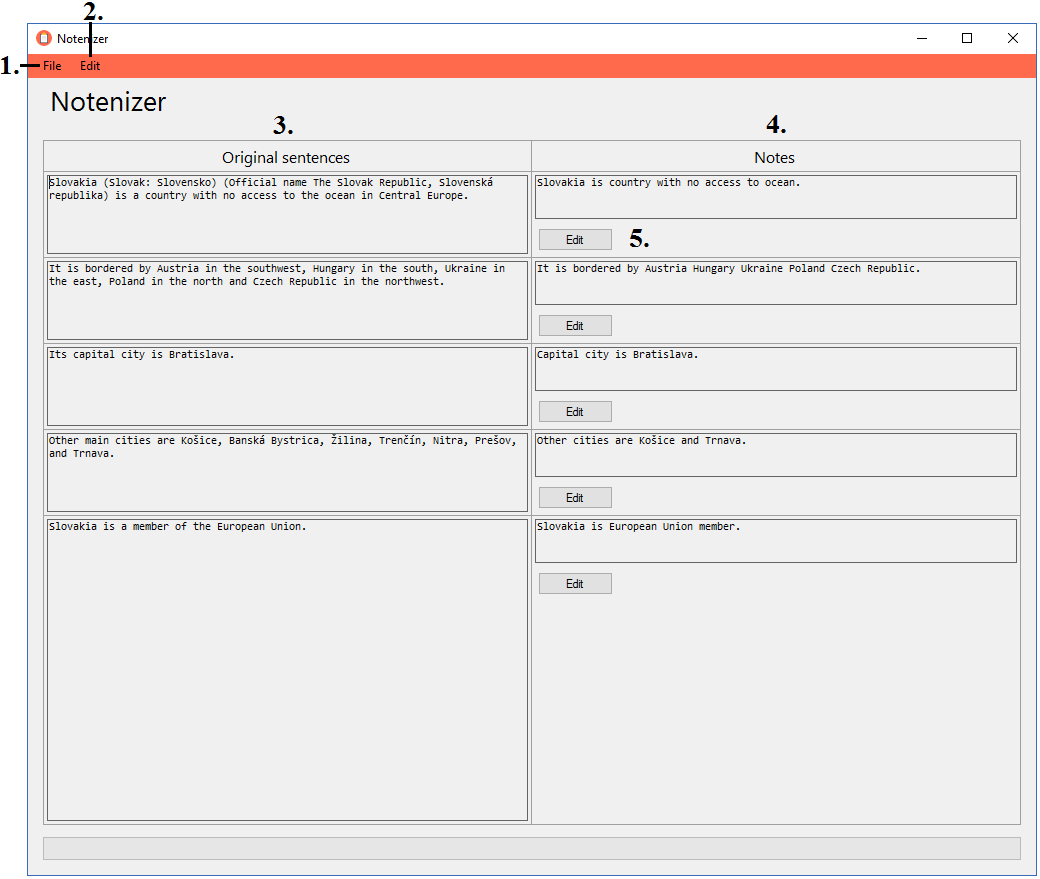
\includegraphics[scale=0.5]{gui_main_window}\end{center}
	\caption[Grafické rozhranie - Hlavné okno]{Grafické rozhranie - Hlavné okno}\label{appendix:gui:main_window}
\end{figure}

Menu File (\imgref{appendix:gui:menu_file}) ponúka viacero operácií s textami:
\begin{my_enumerate}
	\item otvorí okno pre načítanie textu na spracovanie (\imgref{appendix:gui:input_window}),
	\item získa text na spracovanie zo zvoleného textového súboru,
	\item zobrazí okno na stiahnutie textu z wikipédie (\imgref{appendix:gui:link_window}),
	\item uloží vytvorené poznámky do textového súboru,
	\item ukončí program.
\end{my_enumerate}

\begin{figure}[H]
	\begin{center}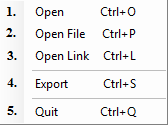
\includegraphics[scale=1]{gui_menu_file}\end{center}
	\caption[Grafické rozhranie - Menu File]{Grafické rozhranie - Menu File}\label{appendix:gui:menu_file}
\end{figure}

Menu Edit (\imgref{appendix:gui:menu_edit}) ponúka operácie:
\begin{my_enumerate}
	\item zo zobrazovacej plochy odstráni pôvodne vety a poznámky.
\end{my_enumerate}

\begin{figure}[H]
	\begin{center}
\includegraphics[scale=1]{gui_menu_edit}\end{center}
	\caption[Grafické rozhranie - Menu Edit]{Grafické rozhranie - Menu Edit}\label{appendix:gui:menu_edit}
\end{figure}

Okno na načítanie textu na spracovanie (\imgref{appendix:gui:input_window}) obsahuje:
\begin{my_enumerate}
	\item textovú plochu na načítanie textu na spracovanie.
\end{my_enumerate}
\begin{figure}[H]
	\begin{center}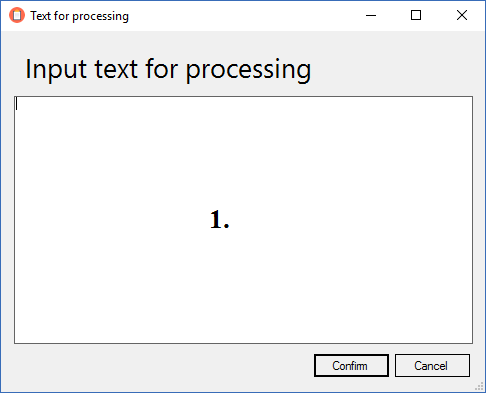
\includegraphics[scale=0.6]{gui_input_text}\end{center}
	\caption[Grafické rozhranie - Okno na načítanie textu]{Grafické rozhranie - Okno na načítanie textu}\label{appendix:gui:input_window}
\end{figure}

Okno na stiahnutie textu (\imgref{appendix:gui:link_window}) sa skladá z:
\begin{my_enumerate}
	\item výber stiahnutia textu cez URL článku na wikipédií,
	\item výber stiahnutia textu z článku na wikipédií podľa názvu krajiny,
	\item zadanie URL alebo názvu krajiny.
\end{my_enumerate}
\begin{figure}[H]
	\begin{center}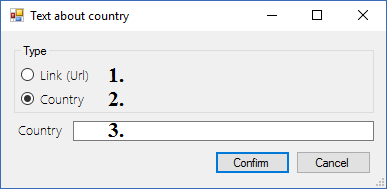
\includegraphics[scale=0.7]{gui_link_window}\end{center}
	\caption[Grafické rozhranie - Okno na dotiahnutie textu]{Grafické rozhranie - Okno na dotiahnutie textu}\label{appendix:gui:link_window}
\end{figure}

Editovacie okno poznámky (\imgref{appendix:gui:edit_window}) obsahuje prvky:
\begin{my_enumerate}
	\item znenie pôvodnej vety,
	\item znenie poznámky,
	\item interaktívne upraviteľný tvar poznámky,
	\item slová z pôvodnej vety, nepoužité v poznámke,
	\item spoznámkovávač viacnásobných poznámok (\imgref{appendix:gui:andparser_window}).
\end{my_enumerate}
\begin{figure}[H]
	\begin{center}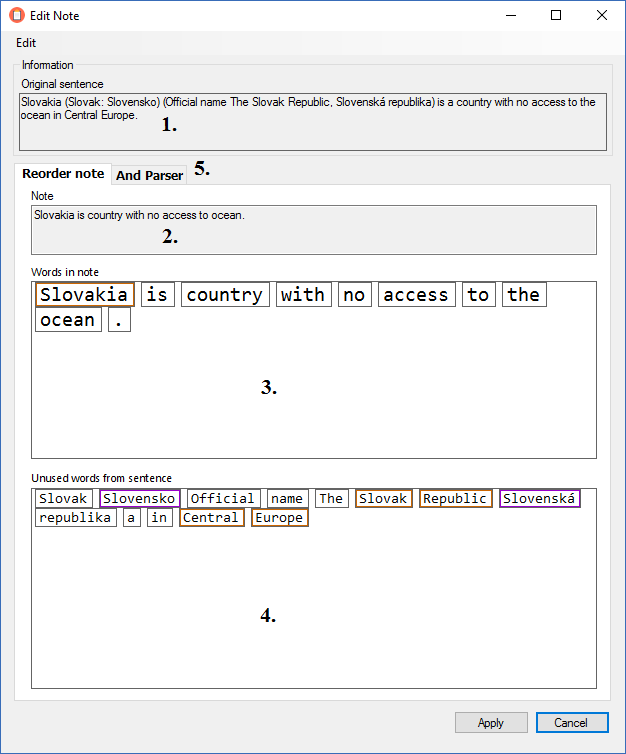
\includegraphics[scale=0.7]{gui_edit_window}\end{center}
	\caption[Grafické rozhranie - Editovacie okno poznámky]{Grafické rozhranie - Editovacie okno poznámky}\label{appendix:gui:edit_window}
\end{figure}

Editovacie okno viacnásobných poznámok (\imgref{appendix:gui:andparser_window}) ponúka:
\begin{my_enumerate}
	\item znenie pôvodnej vety,
	\item viacnásobnú poznámku,
	\item interaktívne upraviteľný tvar viacnásobnej poznámky,
	\item slová z pôvodnej vety, nepoužité vo viacnásobnej poznámke,
	\item špeciálny prvok označujúci množinu viacnásobnej poznámky.
\end{my_enumerate}
\begin{figure}[H]
	\begin{center}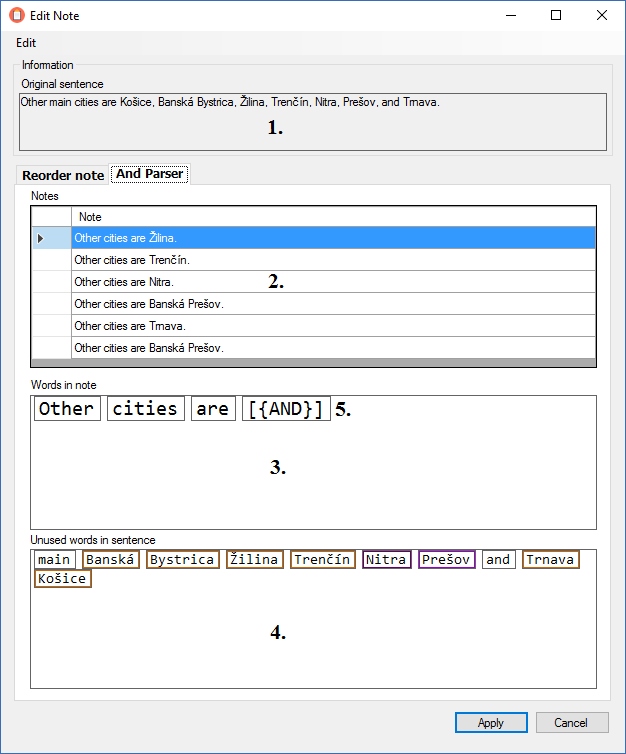
\includegraphics[scale=0.7]{gui_andparser_window}\end{center}
	\caption[Grafické rozhranie - Editovacie okno viacnásobných poznámok]{Grafické rozhranie - Editovacie okno viacnásobných poznámok}\label{appendix:gui:andparser_window}
\end{figure}

\newpage
\ifthenelse {\boolean{bachelor}}
{
	%\section{Electronic medium}
	\section{Electronické médium}
}
{
	%\chapter{Electronic medium}
	\chapter{Electronické médium}
}
Na elektronickom médiu sa nachádza implementácia nášho systému, ako aj zdrojové súbory k implementácií. Vstupné dáta experimentov v textovej podobe aj zálohované z MongoDB databázy. Dostupné sú aj Latex a BibTex zdrojové súbory tejto práce.
\begin{my_itemize}
\emptyitem /Application
	\begin{my_itemize}
	\myitem implementácia opisovaného riešenia
	\end{my_itemize}	
\emptyitem /Documentation
	\begin{my_itemize}
	\myitem bakalárska práca spolu s anotáciami v slovenskom a anglickom jazyku
	\end{my_itemize}
\emptyitem /Documentation/Latex
	\begin{my_itemize}
	\myitem latex zdrojové súbory dokumentácie
	\end{my_itemize}
\emptyitem /Documentation/BibTeX
	\begin{my_itemize}
	\myitem BibTeX súbor s použitými referenciami
	\end{my_itemize}
\emptyitem /Documentation/Resources
	\begin{my_itemize}
	\myitem dostupné použité zdroje
	\end{my_itemize}
\emptyitem /Resources/Data
	\begin{my_itemize}
		\myitem testovacie dáta opisované v dokumente
	\end{my_itemize}
\emptyitem Reqources/Backup
	\begin{my_itemize}
		\myitem zálohované testovacie dáta
	\end{my_itemize}
\emptyitem /Source/Dependencies
	\begin{my_itemize}
	\myitem inštalačné súbory pre knižnice, ktoré potrebuje aplikácia
	\end{my_itemize}	
\emptyitem read.me	- popis obsahu média v slovenskom a~anglickom jazyku
\end{my_itemize}

\newpage
\ifthenelse {\boolean{bachelor}}
{
	%\section{Electronic medium}
	\section{Zoznam vzťahov závislostí}
}
{
	%\chapter{Electronic medium}
	\chapter{Zoznam vzťahov závislostí}
}
V nasledujúcej tabuľke sú zobrazené skratky vzťahov závislostí slov vo vete ako sa používajú v programe, s celým názvom, vysvetlením, príkladom vety a použitím vzhľadom na príkladovú vetu.

\begin{figure}[H]
	\begin{center}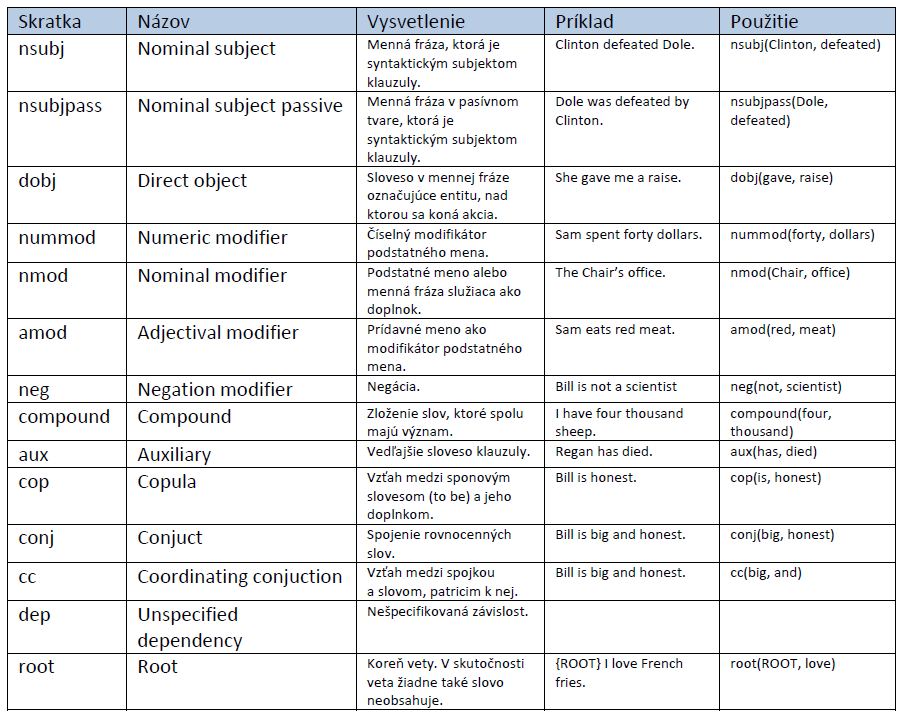
\includegraphics[scale=0.6]{dependencies_table}\end{center}
	\caption[Zoznam závislotí]{Zoznam závislostí}\label{fig:dependencies_table}
\end{figure}

\newpage
\ifthenelse {\boolean{bachelor}}
{
	%\section{Electronic medium}
	\section{Legenda diagramov kolekcií}
}
{
	%\chapter{Electronic medium}
	\chapter{Legenda diagramov kolekcií}
}
V priloženej tabuľke je legenda pre diagramy zobrazujúce štruktúru dát ukladaných v kolekciách v databáze.

\begin{figure}[H]
	\begin{center}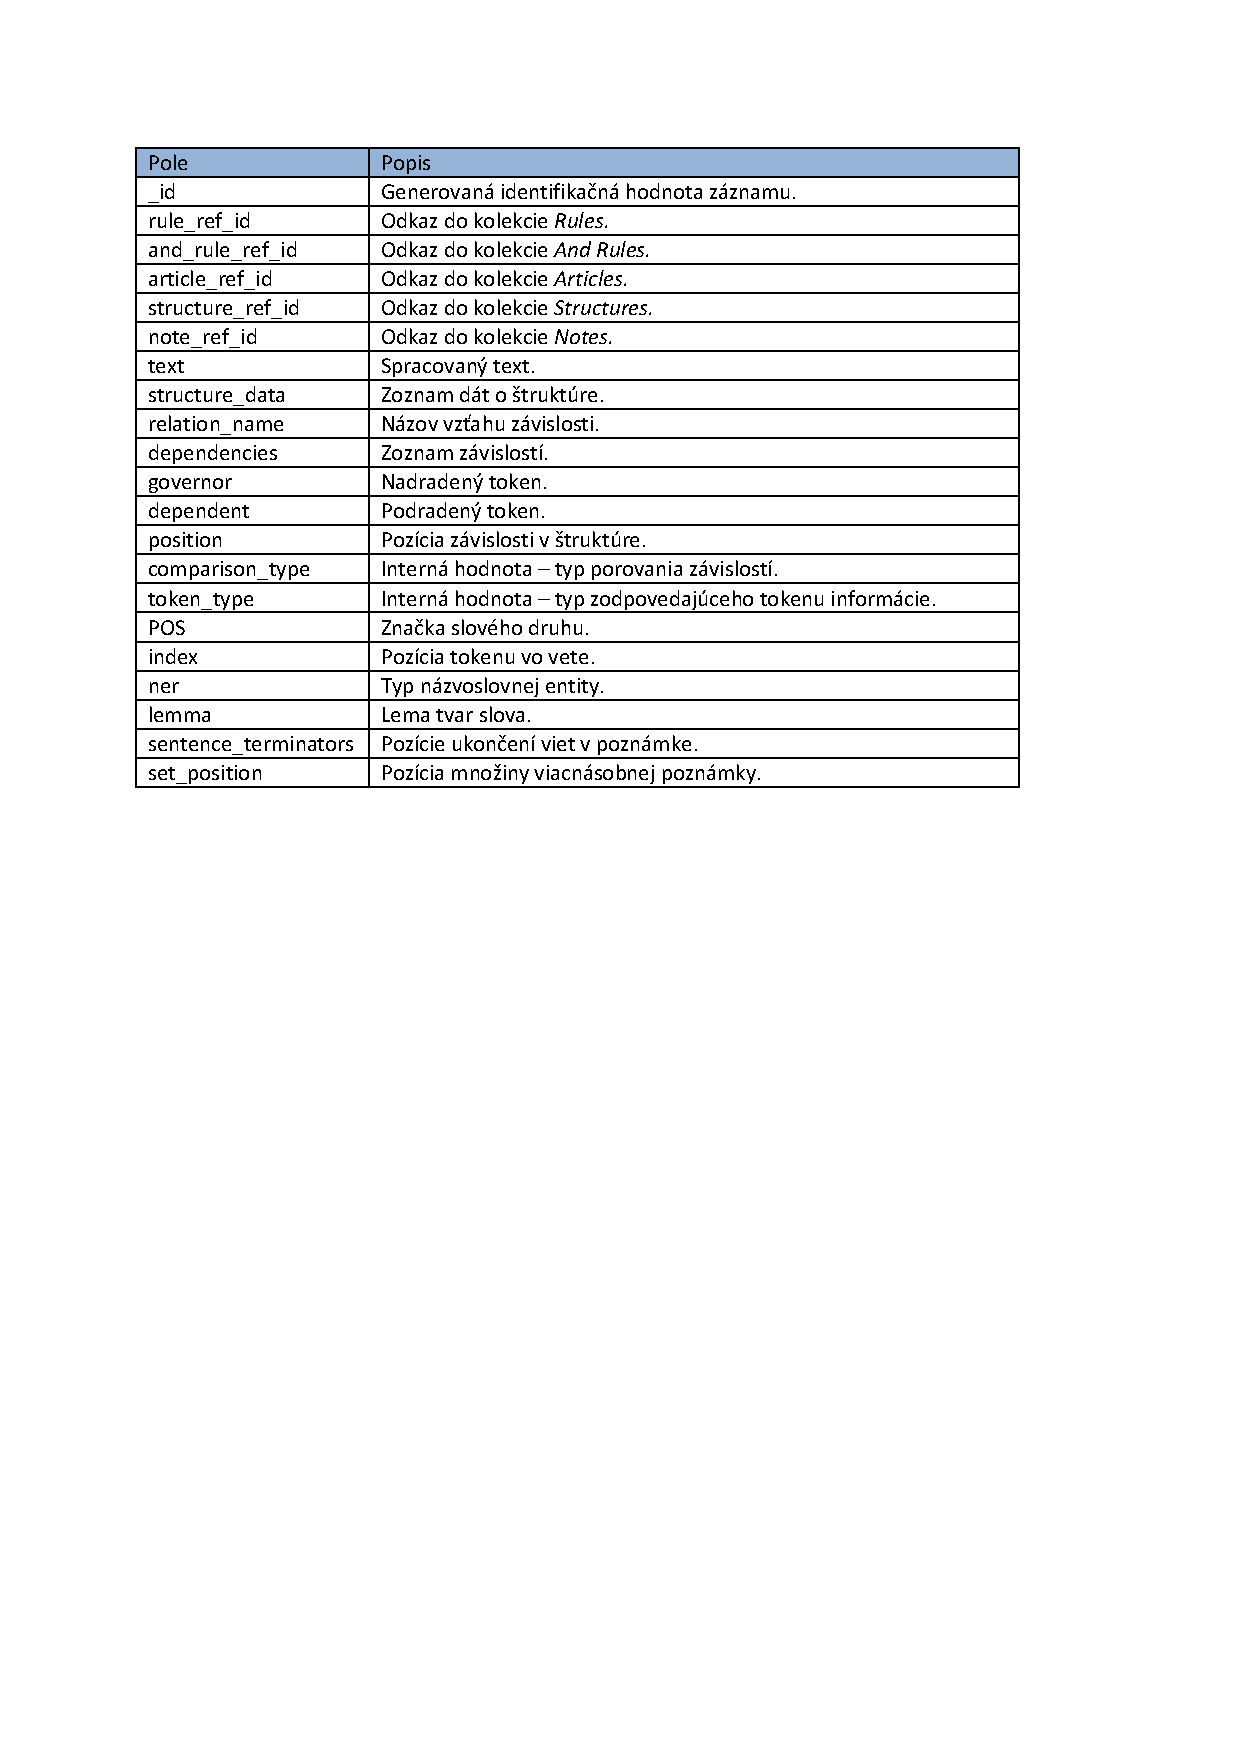
\includegraphics[scale=0.40]{collections_legend}\end{center}
	\caption[Legenda diagramov kolekcií]{Legenda diagramov kolekcií}\label{fig:collections_legend}
\end{figure}

\begin{figure}[H]
	\begin{center}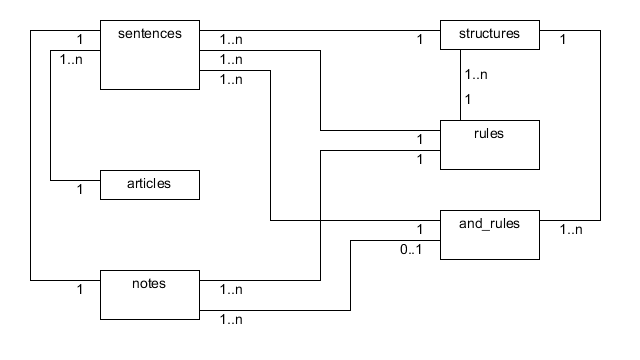
\includegraphics[scale=0.60]{db_schema}\end{center}
	\caption[Databázový model]{Databázový model}
\end{figure}

\begin{figure}[H]
	\begin{center}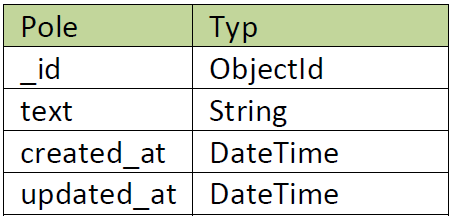
\includegraphics[scale=0.40]{articles_model}\end{center}
	\caption[Model kolekcie articles]{Model kolekcie articles}
\end{figure}

\begin{figure}[H]
	\begin{center}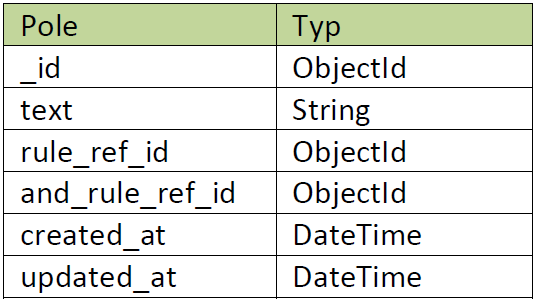
\includegraphics[scale=0.40]{notes_model}\end{center}
	\caption[Model kolekcie notes]{Model kolekcie notes}\label{fig:notes_collection_model}
\end{figure}

\begin{figure}[H]
	\begin{center}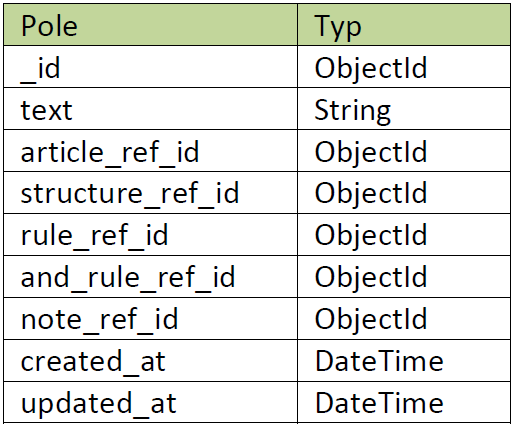
\includegraphics[scale=0.42]{sentences_model}\end{center}
	\caption[Model kolekcie sentences]{Model kolekcie sentences}\label{fig:sentences_collection_model}
\end{figure}

\begin{figure}[H]
	\begin{center}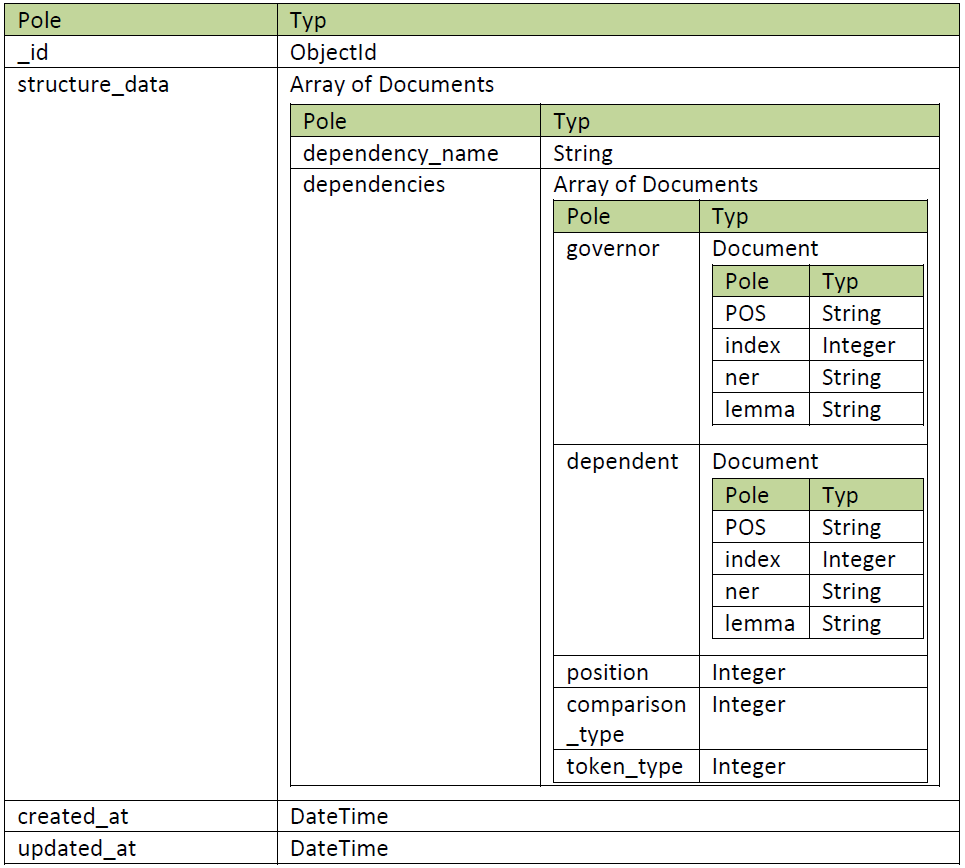
\includegraphics[scale=0.48]{structure_model}\end{center}
	\caption[Model kolekcie structures]{Model kolekcie structures}\label{fig:structures_collection_model}
\end{figure}

\begin{figure}[H]
	\begin{center}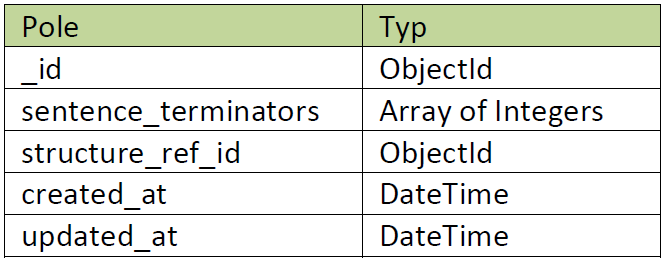
\includegraphics[scale=0.40]{rules_model}\end{center}
	\caption[Model kolekcie rules]{Model kolekcie rules}\label{fig:rules_collection_model}
\end{figure}

\begin{figure}[H]
	\begin{center}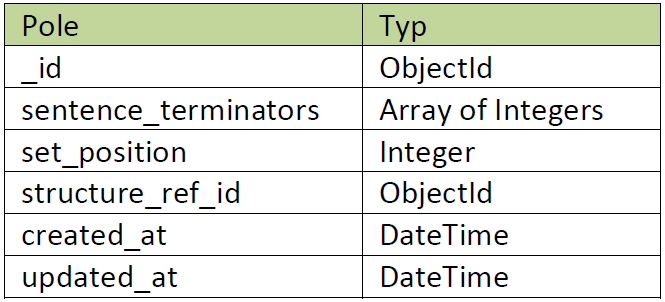
\includegraphics[scale=0.40]{and_rules_model}\end{center}
	\caption[Model kolekcie and rules]{Model kolekcie and rules}\label{fig:and_rules_collection_model}
\end{figure}

\newpage
\ifthenelse {\boolean{bachelor}}
{
	%\section{Electronic medium}
	\section{Ukážka článkov použitých v experimente}
}
{
	%\chapter{Electronic medium}
	\chapter{Legenda diagramov kolekcií}
}
\textit{Slovensko} - ,,Slovakia (Slovak: Slovensko) (Official name The Slovak Republic, Slovenská republika) is a country with no access to the ocean in Central Europe. It is bordered by Austria in the southwest, Hungary in the south, Ukraine in the east, Poland in the north and Czech Republic in the northwest. Its capital city is Bratislava. Other main cities are Košice, Banská Bystrica, Žilina, Trenčín, Nitra, Prešov, and Trnava. Slovakia is a member of the European Union.'' \\

\noindent
\textit{Česko} - ,,Czech Republic (Czech: Česká republika) is a country in Central Europe, sometimes also known as Czechia (Czech: Česko). The capital and the biggest city is Prague. The currency is the Czech Crown (koruna česká - CZK). 1€ is about 27 CZK. The president of the Czech Republic is Miloš Zeman. The Czech Republic's population is about 10.5 million. The local language is Czech language. The Czech language is a Slavic language. It is related to languages like Slovak and Polish. In 1993 the Czech Ministry of Foreign Affairs announced that the name Czechia be used for the country outside of formal official documents. This has not caught on in English usage. Czech Republic has no sea; its neighbour countries are Germany, Austria, Slovakia, and Poland.'' \\

\noindent
\textit{Maďarsko} - ,,Hungary is a country in Central Europe. Its capital city is Budapest. Hungary is slightly bigger than its western neighbour Austria and has about 10 million inhabitants. Other countries that border Hungary are Slovakia, Ukraine, Romania, Serbia, Croatia and Slovenia. Hungary's official language is the Hungarian language. It has been a member of the European Union (EU) since 2004. In Hungarian the country is called Magyarország (Hungary) or Magyar Köztársaság (Hungarian Republic). This is named after the Magyar tribes who came to Hungary in the late 9th century.'' \\

\noindent
\textit{Poľsko} - ,,Poland is a country in Eastern Europe. It is next to Germany to the west (along Oder and Lusatian Neisse), the Czech Republic and Slovakia to the south, Ukraine and Belarus to the east, and the Baltic Sea, Lithuania, and Russia to the north. The total land area of Poland is about 312,679 km2 (120,728 mi2). This makes Poland the 77th largest country in the world with over 38.5 million people. Most Polish people live in large cities, including the capital, Warsaw (Polish: Warszawa), Łódź, Cracow (Polish: Kraków), the second capital of Poland (first was Gniezno), Szczecin, Gdańsk, Wrocław and Poznań. The word "Poland" was written officially for the first time in 966. In 1569, Poland formed a strong union with Lithuania called the Polish-Lithuanian Commonwealth. At some point in its history, it was the largest state in Europe and became very influential. Much of the territory that now makes up Central European states used to belong to the Commonwealth. Eventually, after entering a somewhat sudden yet steady decline, the Commonwealth collapsed in 1795. Poland regained its independence in 1918 after World War I. In 1921, Poland defeated Soviet Russia in the Polish-Soviet War that started in 1919.'' \\

\noindent
\textit{Nemecko} - ,,The Federal Republic of Germany, also called Germany (German: Bundesrepublik Deutschland or just Deutschland), is a country in Central Europe. The country's full name is sometimes shortened to the FRG (or the BRD, in German). To the north of Germany are the North Sea, the Baltic Sea, and the country of Denmark. To the east of Germany are the countries of Poland and the Czech Republic. To the south of Germany are the countries of Austria and Switzerland. To the west of Germany are the countries of France, Luxembourg, Belgium, and the Netherlands. The total area of Germany is 137,847 square miles. The large majority of Germany has warm summers and cool or cold winters. In June 2013, Germany had a population of 80.6 million people. After the United States, Germany is the second most popular country for migration in the world. Before it was called Germany, it was called Germania. In the years A.D. 900 until 1806, Germany was part of the Holy Roman Empire. From 1949 to 1990, Germany was made up of two countries called the Federal Republic of Germany (inf. West Germany) and the German Democratic Republic (inf. East Germany). During this time, the capital city of Berlin was divided into a west and an east part. On 13 August 1961, East Germany started building the Berlin Wall between the two parts of Berlin. West Germany was one of the countries that started the European Union.'' \\

\noindent
\textit{Taliansko} - ,,Italy is a country in Europe and a member of the European Union. Its official name is Repubblica Italiana. Italy is a democratic republic and is a founding member of the European Union. Italy is also a member of the G8, as it has the 8th largest Gross Domestic Product in the world. Its President is Sergio Mattarella and its Prime Minister is Matteo Renzi. Before 1861, it was made up of smaller kingdoms and city-states.'' \\

\noindent
\textit{Francúzsko} - ,,France (French: France), officially the French Republic (French: République française), is a country in Western Europe. Its capital city is Paris. It is a member of the European Union. It is known for its culture, its many monuments and structures, and places such as the Louvre, the Eiffel Tower, the Arc de Triomphe, Giverny, Mont Saint Michel, Versailles, and Notre Dame de Paris. France is divided into 22 régions that are further subdivided départements. The country has been one of the great powers since the end of the 17th century. In the 18th and 19th centuries, it built a big colonial empire across West Africa and Southeast Asia. Nowadays, this does not exist. It is the most visited country in the world. About 82 million foreign tourists visit it every year. France is a founding member of the European Union. It has the largest land area of any member. France is also a founding member of the United Nations, and a member of the G8 and NATO. It is one of the five permanent members of the United Nations Security Council. It has nuclear weapons, including active warheads, and also has nuclear power plants. Some well-known cities in France include Paris, Lyon, Marseille, Bordeaux, Lille, Toulouse, Nice, Strasbourg, Rennes and Nantes.'' \\

\noindent
\textit{Spojené kráľovstvo} - ,,The United Kingdom of Great Britain and Northern Ireland, called the United Kingdom, GB or UK, is a sovereign state in Western Europe. It unites England, Northern Ireland, Scotland and Wales as one Kingdom.[10] It is a member of the European Union, the United Nations, the Commonwealth, NATO and the G8. It has the sixth largest economy in the world. Around 65 million people live in the UK. Most people in the UK speak English. There are five native languages other than English. They are Welsh in Wales, Gaelic and Scots in Scotland and Northern Ireland, Irish in Northern Ireland, and Cornish in Cornwall. Between the 17th and mid 20th-centuries Britain was an important world power. It became a colonial empire that controlled large areas of Africa, Asia, North America and Oceania. Today this empire does not exist, although Britain keeps links with most countries of its former empire. Some well-known cities in the UK are London, Edinburgh, Cardiff, Belfast, Manchester, Bristol, Liverpool, Birmingham, York and Glasgow.'' \\

\noindent
\textit{Španielsko} - ,,Spain is a country in Southern Europe. It is in the Iberian Peninsula near Portugal and Gibraltar. France and the country of Andorra are on its northeast side, where the Pyrenees mountains are. The people of Spain are called Spaniards. Most people there speak Spanish (in Spanish, "Castellano", from Castilla, or "Español") but there are other languages in different parts of the country. They are Catalan, Basque, and Galician, Leonese, Aragonese, Aranese Occitan and even Portuguese. The religion of most of the people in Spain is Roman Catholic. Since 1975, Spain has had a king who only does what the constitution allows him to. For example, the king can declare a war, but only if the Government asks him to do so. The parliament is called Las Cortes Generales, and has two bodies: "El Congreso" (The Congress) and "El Senado" (The Senate) and it is chosen by the Spanish people by voting. This kind of government is called a constitutional monarchy. The King of Spain is Felipe VI. The Prime minister is Mariano Rajoy. The government and the king's palace are in Madrid, the capital of Spain. Spain has more than five hundred thousand square kilometres of land. It is smaller than France, but it is bigger than Sweden or Germany. Almost fifty million people live in Spain. Spain has 17 parts called autonomous communities (this means that they can decide upon some affairs themselves). Each part has its own government.'' \\

\noindent
\textit{Ukrajina} - ,,Ukraine is a country in Eastern Europe. Russia is to the north-east of Ukraine, Belarus is to the Northwest, Poland and Slovakia are to the West, Hungary, Romania, Moldova and self-proclaimed Transnistria are to the South West and the Black Sea is to the Southwest. Ukraine is a republic. The capital of Ukraine is Kiev. It was a part of the Soviet Union from 1922 until 1991.'' \\

\noindent
\textit{Rakúsko} - ,,Austria (German: Österreich; officially called Republic of Austria), is a country in Central Europe. Around Austria there are Germany, Czech Republic, Slovakia, Hungary, Slovenia, Italy, Switzerland, and Liechtenstein. Currently, the chancellor is Werner Faymann. Austria has been a member-state of the EU since 1995. The people in Austria speak German, a few also Hungarian, Slovenian and Croatian. The capital of Austria is Vienna (Wien). Austria is more than a thousand years old. Its history can be followed to the ninth century. At that time the first people moved to the land now known as Austria. The name "Ostarrichi" is first written in an official document from 996. Since then this word has developed into the Modern German word Österreich, which literally means "East Kingdom." Austria is a democratic state and has nine federal states (German: 'Bundesländer'): Vorarlberg, the Tyrol, Salzburg, Carinthia, Styria, Upper Austria, Lower Austria, Vienna and Burgenland. It is a neutral state, that means it does not take part in wars with other countries. Austria has been in the United Nations since 1955 and in the European Union since 1995.'' \\

\noindent
\textit{Švédsko} - ,,Sweden (Swedish: Sverige) is a Nordic country in the part of Europe called Scandinavia. Its neighbors are Finland and Norway. Sweden is also connected to Denmark in the south by a bridge. It is a developed country. It is famous for its welfare state. People who live in Sweden are called Swedes. Sweden's capital city is Stockholm. Sweden is a constitutional monarchy because it has a king, Carl XVI Gustaf, but he does not have any real power. Sweden is a parliamentary state meaning that the government is elected by the parliament which is appointed by the people. The country is democratically ruled by a government headed by an elected prime minister. Stefan Löfven was elected Prime Minister in September 2014. He took office in October 2014. The population of Sweden is almost 9.5 million people. Sweden has an official majority language, (called svenska in Swedish). Sweden has five official minority languages, Finnish, Yiddish, Sami, Meänkieli and Romani. Sweden became a member of the European Union in 1995. It is not a member of the Eurozone. Sweden has not begun to use the euro as currency. This is because the people have voted against this. The currency remains the Swedish krona (Swedish crown). Sweden has 25 provinces (landskap). They are found in three different regions: Norrland in the North, Svealand, the central region, and Götaland in the South.''

\newpage
\ifthenelse {\boolean{bachelor}}
{
	%\section{Electronic medium}
	\section{IIT.SRC článok}
}
{
	%\chapter{Electronic medium}
	\chapter{Legenda diagramov kolekcií}
}
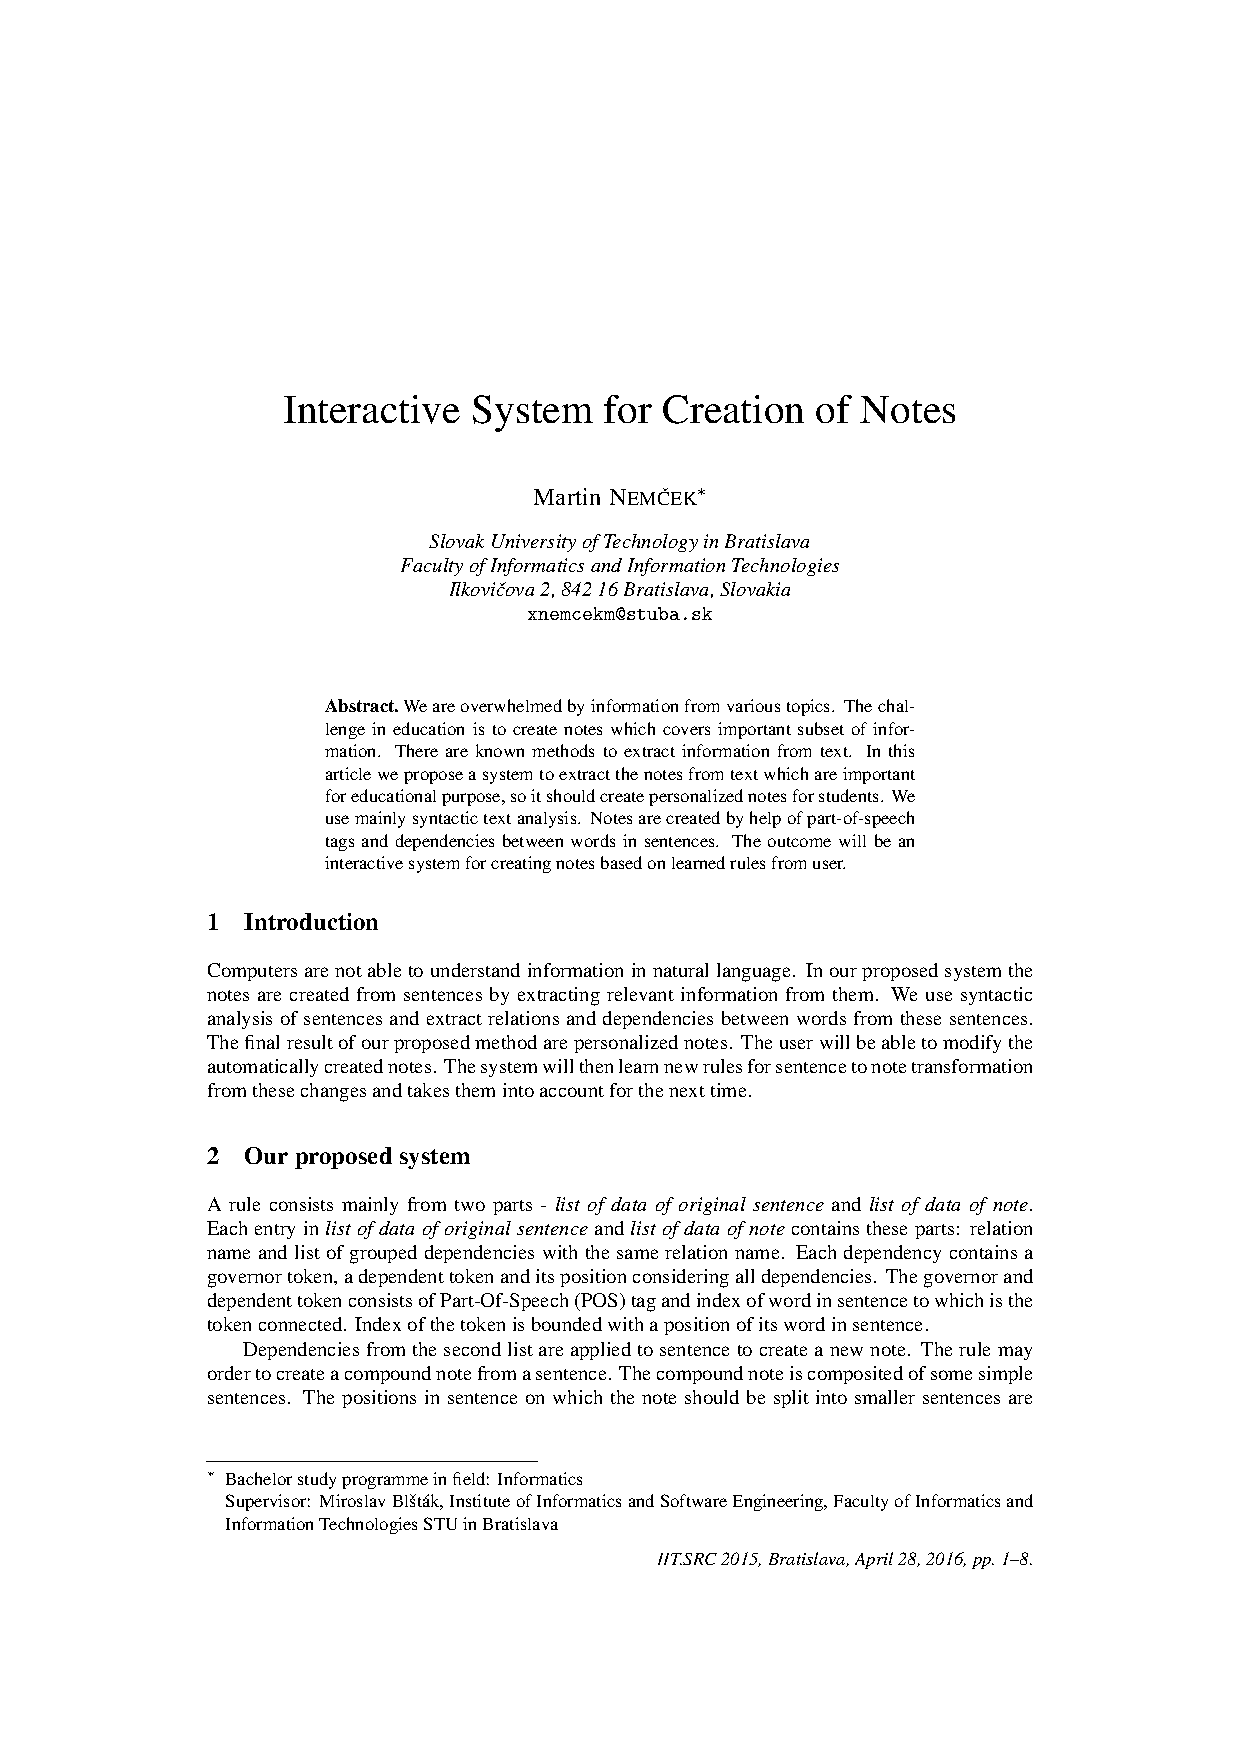
\includepdf[pages={1,2,3}, pagecommand={}]{interactive_system_for_creation_of_notes.pdf}
\afterpage{\null\newpage}
